% ===== 原文 pp.30--33 =====

% [原文 p.30]
\section{class S 理论的拉格朗日量}

在讨论了管子收缩时出现的驯服穿刺点之后，我们在 4.1 小节论证：球面上带三个驯服穿刺点的 $\cX(\fsu(2))$ 给出 4 个自由超多重态，并把味对称性 $\mathrm{SU}(2)^3$ 显现出来。在 4.2 小节我们把两个这样的构件粘起来，以了解带四个驯服穿刺点的球面上的 $\cX(\fsu(2))$ 如何重现规范群为 $\mathrm{SU}(2)$、$N_f=4$ 的 4d $\cN=2$ SQCD 的已知性质。这是 AGT 综述的传统起点：人们通常先研究 $\mathrm{SU}(2)$ SQCD 的 S 对偶 [4] 与箭图规范理论的 S 对偶 [175]，然后再解释统一的 6d 观点 [1]。我们在 4.3 小节把讨论推广到由任意带穿刺黎曼面上的 $\cX(\fsu(2))$ 所产生的广义 $\mathrm{SU}(2)$ 箭图。

\begin{keybox}{穿刺点的描述与几个 tinkertoy}
\begin{itemize}[leftmargin=1.4em,itemsep=1pt,topsep=1pt]
  \item $\fsu(2)$ 的 tinkertoy 由一个 $\mathrm{SU}(2)^3$ 三基本表示（trifundamental）半超多重态组成。
  \item 带两个满驯服穿刺点与一个单驯服穿刺点的 $\fsu(N)$ tinkertoy 是一个 $\mathrm{SU}(N)^2$ 双基本表示超多重态。
  \item 对 $\fsu(N)$，在满驯服穿刺点 $z_0$ 处各微分满足
        $\phi_k=\left(\frac{\sigma_k}{(z-z_0)^k}+O\!\left(\frac{1}{(z-z_0)^{k-1}}\right)\right)\dd z^k$
        （$2\le k\le N$），其中 $\sigma_k$ 的质量量纲为 $k$。其他的驯服穿刺点由把极点系数限制到低于 $k-1$ 的阶而得到。
  \item 许多线性箭图既有 class S 描述也有 IIA 描述；Coulomb 分支与 SW 曲线都相符。
\end{itemize}
\end{keybox}

% [Tutor Note: p.30 要点框。术语首现：full tame puncture = 满驯服穿刺点（留数取“最大可能阶”$k$ 的极点），simple tame puncture = 单驯服穿刺点。核对 $\sigma_k$ 的量纲：$\phi_k=\langle\cO_k\rangle$ 是 $k$ 次微分，$\dd z^k$ 量纲为 $-k$，故 $\sigma_k$ 量纲为 $k$；与 $\phi_2=\frac12\Tr(\phi^2)\dd z^2$ 中 $m^2$ 的量纲 2 一致。]

在 4.4 小节我们把一些 $\mathrm{SU}(N)$ 线性箭图规范理论（包括 $N_f=2N$ 的 $\mathrm{SU}(N)$ SQCD）实现为 class S 理论。这告诉我们：驯服穿刺点有若干类型，因而 6d 理论中有若干类型的余维 4 算子。本节考虑的所有理论都满足规范耦合的单圈 beta 函数为零，而这蕴涵耦合在所有阶的 beta 函数都为零 [176]。

% [Tutor Note: p.30 原文“and of quivers gauge theories [175]”中 “quivers” 应为 “quiver”（quiver gauge theories，箭图规范理论），属笔误；此处按正确形式译作“箭图规范理论”。]

\subsection{三基本表示 tinkertoy}

我们来讨论驯服穿刺点；对 $\fsu(2)$ 只有一种类型。然后考虑 $\C P^1$ 球面上在 $0,1,\infty$ 处带三个驯服穿刺点的 $\cX(\fsu(2))$，并论证所得的 tinkertoy $T_2=T_{\fsu(2)}$（它是 $\fsu(2)$ class S 理论的主要构件）是四个自由超多重态的集合。这个事实没有第一性原理的推导，但我们会看到对它的许多检验，尤其是对许多规范理论的 Coulomb 分支与 SW 曲线的正确“回推”（postdiction），以及与弦论对偶性的相容性。

% [Tutor Note: p.30 原文用 postdiction（回推）而非 prediction（预言）：作者明言“没有第一性原理推导”，所以这里的检验只能是拿已知的 SW 曲线/对偶性反推确认 $T_2$ 的识别是否正确（见 p.37 对 [123] 的对照）。]

% [原文 p.31]
\para{驯服穿刺点。} 我们通过穿刺点对刻画 Coulomb 分支的 Hitchin 场 $\phi(z)$ 的影响来描述它们，或者以规范不变的方式用高阶微分 $\phi_{d_k}$（$k=1,\dots,\rank\fg$）来描述。

穿刺点可以来自细管子的收缩。在描述这根管子的复坐标 $w\in\R\times S^1$ 中，$\phi_{d_k}$ 在细管子内部往往趋于常数（乘以 $\dd w^{d_k}$）。把柱面切开（与 (3.18) 中所做的相反）并应用指数映照 (3.17) $z=\ee^{w}$，我们一般预期
\begin{equation}
  \phi_{d_k}\simeq\frac{\dd z^{d_k}}{z^{d_k}}+\cdots
  \tag{4.1}
\end{equation}
附带某些系数，其中所用局部坐标 $z$ 使穿刺点在 $z=0$。

% [Tutor Note: p.31 式 (4.1) 的推导要点：管子里 $\phi_{d_k}\simeq c\,\dd w^{d_k}$ 为常数，代入 $w=\log z$ 得 $\dd w=\dd z/z$，故 $\phi_{d_k}\simeq c\,(\dd z/z)^{d_k}=c\,\dd z^{d_k}/z^{d_k}$------这正是 $d_k$ 阶极点、首项系数为 $c$。核对指标 $d_k$：原文用 $d_k$ 表示 $\fg$ 的各基本不变式的次数（$\fsu(N)$ 时为 $2,\dots,N$），与要点框中写的 $k$ 是同一件事。]

这促使我们使用\textit{驯服穿刺点}（tame puncture），即 $\phi(z)\dd z$ 具有给定留数的一阶极点的点（当然要在规范共轭意义下）：给定的留数一般翻译为 (4.1) 中给定的首项系数------这就是一个\textit{满}驯服穿刺点。其他类型的穿刺点我们将在第 7 节研究：$\phi_{d_k}$ 具有比 (4.1) 更低阶极点的驯服穿刺点，以及定义为具有更高阶极点的野生穿刺点。

\para{$\fsu(2)$ 的有质量与无质量驯服穿刺点。} 目前我们先聚焦于 $\fsu(2)$：此时只有一种类型的驯服穿刺点。

这种情形只有一个 Casimir，即二次微分 $\phi_2=\frac12\Tr(\phi^2)\dd z^2$。我们把 Hitchin 场 $\phi$ 的留数在共轭意义下定死（记作 $\sim$）：对非零的 $m\in\C$，
\begin{equation}
  \phi(z)\sim\left(\frac{\diag(m,-m)}{z-z_i}+O(1)\right)\dd z
  \quad\Longrightarrow\quad
  \phi_2(z)=\left(\frac{m^2}{(z-z_i)^2}+O\!\left(\frac{1}{z-z_i}\right)\right)\dd z^2.
  \tag{4.2}
\end{equation}
我们把 $m\neq 0$ 称为该穿刺点的\textit{质量参数}，理由如下。由 (3.15) 定义的 $\Sigma$ 的各片行为是 $x_\pm(z)=\pm m/(z-z_i)+O(1)$，而把 SW 微分 $\lambda$ 绕 $z_i$ 在 $\Sigma$ 的一片上积分会拾取留数 $\pm m$。这意味着 $m$ 作为对中心荷的一项贡献出现，从而也是对 BPS 粒子质量的一项贡献。

天真地，在 $\phi(z)$ 的渐近式中取 $m\to 0$ 极限会把 $z_i$ 变成一个正则点。然而在 $\phi_2$ 的方程中，穿刺点仍以一阶极点存在。从 $\phi(z)$ 的角度看，这可以由下述事实解释：它只在共轭意义下才有定义。在取 $m\to0$ 极限之前对对角矩阵 $\diag(m,-m)$ 作共轭，可以得到非零的值，
\begin{equation}
  \begin{pmatrix} m & 0 \\ 0 & -m \end{pmatrix}
  \sim
  \begin{pmatrix} m & 1 \\ 0 & -m \end{pmatrix}
  \xrightarrow{\ m\to 0\ }
  \begin{pmatrix} 0 & 1 \\ 0 & 0 \end{pmatrix}.
  \tag{4.3}
\end{equation}
确实，我们得到一个自洽的\textit{无质量}驯服穿刺点
\begin{equation}
  \phi(z)\sim\left(\begin{pmatrix} 0 & 1 \\ 0 & 0 \end{pmatrix}\frac{1}{z-z_i}+O(1)\right)\dd z
  \quad\Longrightarrow\quad
  \phi_2(z)=O\!\left(\frac{1}{z-z_i}\right)\dd z^2
  \tag{4.4}
\end{equation}
其中极点的系数是自由的。有趣的是，由 $x^2\dd z^2=\phi_2$ 定义的 $\Sigma$ 的各片在这样的无质量穿刺点处有一个分支点。

% [Tutor Note: p.31 式 (4.3)--(4.4) 的核对办法：取 $N=\begin{pmatrix}0&1\\0&0\end{pmatrix}$，则 $N^2=0$，故 $\Tr(N^2)=0$，于是 $\phi_2=\frac12\Tr(\phi^2)\dd z^2$ 在 $z_i$ 处的二阶极点系数（即 $m^2$）恰为零，只剩一阶极点------这正是 (4.4) 与 (4.3) 相容的原因，也说明为何“无质量”对应幂零矩阵。逆推检查：若把 (4.3) 中的 $\begin{pmatrix}m&1\\0&-m\end{pmatrix}$ 直接代入 $\frac12\Tr(\phi^2)$ 会得 $\frac12(m^2+(-m)^2)=m^2$，再取 $m\to0$ 得 0，与 (4.4) 的首项一致。]

% [原文 p.32]
\begin{exercise}{4.1}
1. 对任意 $\alpha\in\C$，找出可逆矩阵 $g\in\mathrm{SL}(2,\C)$，使得 $g^{-1}\diag(m,-m)\,g=\begin{pmatrix} m & \alpha \\ 0 & -m\end{pmatrix}$。

2. 验证所有 $\begin{pmatrix} 0 & \alpha \\ 0 & 0\end{pmatrix}$（$\alpha\neq 0$）彼此共轭。

3. (4.2) 与 (4.4) 中 $1/(z-z_i)$ 的系数，是如何由 $\phi$ 的展开式中 $(z-z_i)^0$ 项的各分量产生的？
\end{exercise}

我们把 (4.2) 解释如下：无质量穿刺点 (4.4) 带有 $\mathrm{SU}(2)$ 味对称性，而在与该对称性耦合的背景矢量多重态中开启常数标量 $\phi_{\text{background}}=m$，就会把该穿刺点变成有质量的 (4.2)。

% [Tutor Note: p.32 这一段是 punctures 与 flavour symmetry 的桥梁：$\phi_{\text{background}}$ 是背景矢量多重态标量，其真空期望值即质量参数；把 (4.2) 的留数写成 $\diag(m,-m)$ 等价于给该 $\mathrm{SU}(2)$ 味对称性一个质量形变。后面 4.2 节把 $m_1,m_2,m_3,m_4$ 当作四个穿刺点的质量参数，用的正是这一解释。]

\para{三孔球面与对称性。} 现在考虑 $T_2$，即把 $\cX(\fsu(2))$ 放在带三个驯服穿刺点的球面 $\C P^1$ 上的结果。关于 $T_2$，我们确切知道些什么？

首先，它至少有 $\mathrm{SU}(2)^3$ 味对称性，即每个穿刺点一个 $\mathrm{SU}(2)$。我们在下一个习题中将学到，4 个自由超多重态确实有 $\mathrm{USp}(8)$ 味对称性，它包含 $\mathrm{SU}(2)\times\mathrm{Spin}(4)=\mathrm{SU}(2)^3$。在这个语境下，$\mathrm{USp}(8)$ 味对称性是一种涌现（emergent）对称性：它只在 $C$ 收缩为一点的极限下存在，并不是 6d 设置的对称性。

\begin{exercise}{4.2}
1. 验证 $k$ 个自由标量场带有 $O(k)$ 味对称性。验证 $p$ 个自由超多重态含有 $4p$ 个自由标量，因而有 $O(4p)$ 对称性（此外还有来自旋量的对称性）。在这些对称性中验证：存在一个 $\mathrm{USp}(2p)$ 子群与 $\mathrm{SU}(2)_R$ R 对称性对易。（提示：作为中间步骤，$\mathrm{U}(2p)$ 子群与 $J_3\in\mathrm{SU}(2)_R$ 对易。）

2. 现在把对角嵌入 $\mathrm{USp}(2)^p\subset\mathrm{USp}(2p)$ 的 $\mathrm{SU}(2)=\mathrm{USp}(2)$ 味对称性规范化。被规范化的 $\fsu(2)$ 与 $\fsu(2)_R$ 合成 $\fso(4)$。验证这 $4p$ 个标量组织成 $p$ 份 $\fso(4)$ 基本表示。由此推出剩余的味对称性是 $\mathrm{SO}(p)$。由于超多重态中旋量的作用，它实际上是 $\mathrm{Spin}(p)$。
\end{exercise}

\para{三基本表示半超多重态。} 四个超多重态的三个 $\mathrm{SU}(2)$ 对称性可以全部显现出来，代价是把 $\cN=2$ 超对称隐藏起来。把每个超多重态拆成一对 $\cN=1$ 手征多重态 $(q,\tilde q)$。四个超多重态便拆成八个 $\cN=1$ 手征多重态 $q_{aiu}$，其中 $a,i,u$（取值 $1$ 到 $2$）是三个独立 $\mathrm{SU}(2)$ 的指标。为了把超多重态重构为 $(q,\tilde q)$，只需引入记号
\begin{equation}
  \tilde q^{aiu}=\epsilon^{ab}\epsilon^{ij}\epsilon^{uv}q_{bjv}.
  \tag{4.5}
\end{equation}
因此超多重态处于 $\mathrm{SU}(2)^3$ 的三基本表示中，并带有把独立分量数目减半的实在性条件 (4.5)。这组物质场称为半超多重态。

如果为三个 $\mathrm{SU}(2)$ 开启背景矢量多重态标量（即质量 $m_1,m_2,m_3$），则底层的 8 个手征多重态具有复质量 $\pm m_1\pm m_2\pm m_3$（对一切符号选择）。特别地，当 $m_2=\pm m_1\pm m_3$ 时，4 个超多重态之一变成无质量的。这一点在后面很重要。

% [Tutor Note: p.32 式 (4.5) 的核对：右侧 $\epsilon^{ab}\epsilon^{ij}\epsilon^{uv}$ 三个反对称张量把三个 $\mathrm{SU}(2)$ 指标分别收缩，$q_{bjv}$ 全降指标而 $\tilde q^{aiu}$ 全升，故 (4.5) 是 $\mathrm{SU}(2)^3$ 不变的；对每个 $(a,i,u)$ 作两次变换回到自身（$\epsilon^{ab}\epsilon_{bc}=-\delta^a{}_c$），故它是“实在性条件”、恰好把 $2^3=8$ 个复分量减半为 4 个超多重态的 4 个复标量。质量谱验算：$\pm m_1\pm m_2\pm m_3$ 共 8 个符号组合，正是 8 个 $\cN=1$ 手征多重态的复质量；而按超多重态（每对 $(q,\tilde q)$）配对后给出 4 个质量。]

% [原文 p.33]
\para{$T_2$ 的 Seiberg--Witten 曲线。} 我们把 $0,1,\infty$ 处穿刺点的质量参数（在 (4.2) 或 (4.4) 的意义下）记为 $m_1,m_2,m_3$。\footnote{在目前这个阶段，我们还不知道它们与上一段关于三基本表示半超多重态的那组参数是同一组参数。} 该 4d 理论的 Coulomb 分支（若存在）由全纯二次微分 $\phi_2(z)$ 参数化：这些微分在每个穿刺点处具有二阶极点 (4.2)（无质量情形下为一阶 (4.4)），且没有其他极点。无穷远处的穿刺点翻译为 $z\to\infty$ 时的条件：
\begin{equation}
  \phi_2(z)=\left(\frac{m_3^2}{z^2}+O\!\left(\frac{1}{z^3}\right)\right)\dd z^2.
  \tag{4.6}
\end{equation}
我们回忆关于整函数的 Liouville 定理（$C$ 上处处没有极点的全纯函数）：若整函数 $f$ 有界为 $|f(z)|<Kz^p$（$K$ 为常数、$p$ 为指数），则 $f$ 是次数至多为 $p$ 的多项式。

\begin{exercise}{4.3}
找出具有 $0,1,\infty$ 处规定的二阶极点、且没有其他奇点的二次微分 $\phi_2(z)=u_2(z)\dd z^2$，并证明它唯一。（提示：把它写成 $u_2(z)=f(z)/(z^2(z-1)^2)$，换到 $w=1/z$ 变量以在无穷远处多项式地界定 $f$，用 Liouville 定理限定 $f$ 的次数，然后与规定的渐近式比较以定出系数。）
\end{exercise}

于是 Coulomb 分支是单独一个点，这与我们把 $T_2$ 描述为自由超多重态时没有矢量多重态相一致。具体地，
\begin{equation}
  \phi_2(z)=u_2(z)\dd z^2,
  \qquad
  u_2(z)=\frac{-m_1^2}{z^2(z-1)}+\frac{m_2^2}{z(z-1)^2}+\frac{m_3^2}{z(z-1)}.
  \tag{4.7}
\end{equation}

% [Tutor Note: p.33 式 (4.7) 的三处渐近核对（这是最快的验证法）：$z\to0$ 时首项 $(-m_1^2)/(z^2\cdot(-1))=m_1^2/z^2$ ✓；$z\to1$ 时首项 $m_2^2/(1\cdot(z-1)^2)=m_2^2/(z-1)^2$ ✓；$z\to\infty$ 时 $-m_1^2/z^3+m_2^2/z^3+m_3^2/z^2+O(z^{-3})$，首项 $m_3^2/z^2$ ✓，与 (4.6) 一致。]

让我们求 $T_2$ 在这个唯一 Coulomb 分支真空上的 IR 描述。正如我们在第 24 页评论过的，低能理论一般是 4d $\cN=2$ 阿贝尔规范理论，其矢量多重态标量生活在 Coulomb 分支 $\cB$ 中。这里没有 Coulomb 分支，因而 IR 中没有规范场。但可能有超多重态：为此我们必须研究由 $x^2=u_2$ 定义的 SW 曲线 $\Sigma$ 以及 SW 微分 $\lambda=x\,\dd z$。$\lambda$ 在闭圈上的积分告诉我们 BPS 态的质量。

曲线 $\Sigma$ 是 $\C P^1$ 的分歧二重覆盖。它有多少个分支点？分支点是两片 $x=\pm\sqrt{u_2}$ 重新接合的地方，即 $u_2=0$ 的地方。这发生在二次多项式（一般地）的两个根处，
\begin{equation}
  z^2(z-1)^2u_2(z)=-(z-1)m_1^2+z\,m_2^2+z(z-1)m_3^2.
  \tag{4.8}
\end{equation}
总之，$\Sigma$ 绕球面两圈，只有一条分支割线。因此它在拓扑上是一个球面。$0,1,\infty\in\C P^1$ 处的三个穿刺点在 $\Sigma$ 上变成六个点，SW 微分 $\lambda$ 在那里发散：
% [Tutor Note: p.33 原文“become six point on $\Sigma$”中 “point” 应为复数 “points”（p.36 同处亦然：“hence eight point on $\Sigma$”）；此处按正确语法译作“六个点”“八个点”。]
\begin{equation}
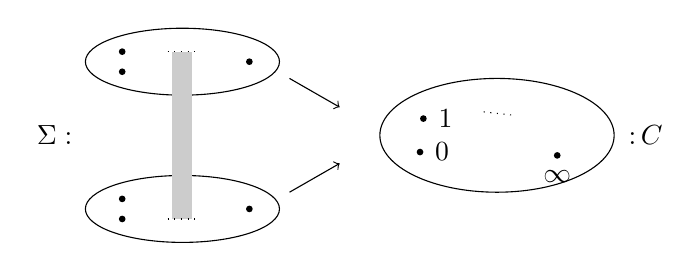
\begin{tikzpicture}[scale=0.85,baseline=(current bounding box.center)]
  \draw (1.6,1.1) ellipse (1.45 and 0.5);
  \fill (0.7,1.25) circle (0.05);
  \fill (0.7,0.95) circle (0.05);
  \fill (2.6,1.1) circle (0.05);
  \draw (1.6,-1.1) ellipse (1.45 and 0.5);
  \fill (0.7,-0.95) circle (0.05);
  \fill (0.7,-1.25) circle (0.05);
  \fill (2.6,-1.1) circle (0.05);
  \draw[fill=gray!40,draw=none] (1.45,-1.25) rectangle (1.75,1.25);
  \draw[dotted] (1.38,1.25)--(1.82,1.25);
  \draw[dotted] (1.38,-1.25)--(1.82,-1.25);
  \node[left] at (0.1,0) {$\Sigma:$};
  \draw[->] (3.2,0.85)--(3.95,0.42);
  \draw[->] (3.2,-0.85)--(3.95,-0.42);
  \draw (6.3,0) ellipse (1.75 and 0.85);
  \fill (5.2,0.25) circle (0.05);
  \node[right] at (5.28,0.25) {$1$};
  \fill (5.15,-0.25) circle (0.05);
  \node[right] at (5.23,-0.25) {$0$};
  \fill (7.2,-0.3) circle (0.05);
  \node[below] at (7.2,-0.38) {$\infty$};
  \draw[dotted] (6.1,0.35)--(6.55,0.3);
  \node[right] at (8.12,0) {$\colon C$};
\end{tikzpicture}
\tag{4.9}
\end{equation}

% [Tutor Note: p.33 式 (4.9) 的线描图（$\Sigma$ 作为 $\C P^1$ 的分歧二重覆盖，灰色带为分支割线）按 STYLE_GUIDE 6bis 用 TikZ 重画，标签 $0,1,\infty$ 与 $\Sigma$、$C$ 照抄原图。与 (4.8) 的核对：$z^2(z-1)^2u_2(z)$ 是二次多项式（两个根 = 两个分支点），对应图中灰色带的一个端点对；六个点是三个穿刺点各在 $\Sigma$ 的两片上各出一份（$3\times2=6$），与正文“六个点”一致。]
